\documentclass[epsfig,a4paper,11pt,titlepage,oneside,openany]{book}
\usepackage{epsfig}
\usepackage{plain}
\usepackage{setspace}
\usepackage[paperheight=29.7cm,paperwidth=21cm,outer=2cm,inner=2cm,top=2cm,bottom=2cm]{geometry}
\usepackage{titlesec} % per formato custom dei titoli dei capitoli

\usepackage{hyperref}
\usepackage{listings}

\usepackage{graphicx}
\graphicspath{ {./images/} }

\begin{document}


\pagenumbering{gobble}

% Pagina iniziale
\pagestyle{plain}

\thispagestyle{empty}

\begin{center}
  \begin{figure}[h!]
    \centerline{
\psfig{file=marchio_unitrento_colore_it_202002.eps,width=0.6\textwidth}}
  \end{figure}

  \vspace{2 cm} 

  \LARGE{Department of Information Engineering and Computer Science\\}

  \vspace{1 cm} 
  \Large{NETWORK SECURITY\\LABORATORY REPORT}

  \vspace{2 cm} 
  \vspace{1 cm} 
  \Huge\textsc{LAB 10\\HONEYPOT}


  \vspace{2 cm} 
  \begin{tabular*}{\textwidth}{ c @{\extracolsep{\fill}} c }
  \Large{Da Rold Giovanni}& \Large{Meschini Marcello}\\
  \Large{224291}& \Large{220222}\\
  \end{tabular*}

  \vspace{2 cm} 

  \Large{Academic year 2020/2021}
  
\end{center}
\clearpage

\pagestyle{plain}
\mainmatter
% indice
\tableofcontents
\clearpage
    
    
          
% gruppo per definizone di successione capitoli senza interruzione di pagina
\begingroup
% nessuna interruzione di pagina tra capitoli
% ridefinizione dei comandi di clear page
\renewcommand{\cleardoublepage}{} 
\renewcommand{\clearpage}{} 
\titleformat{\chapter}
  {\normalfont\Huge\bfseries}{\thechapter}{1em}{}
  
\titlespacing*{\chapter}{0pt}{0.59in}{0.02in}
\titlespacing*{\section}{0pt}{0.20in}{0.02in}
\titlespacing*{\subsection}{0pt}{0.10in}{0.02in}

\chapter*{Info about the lab} % senza numerazione
\label{info}

\addcontentsline{toc}{chapter}{Info about the lab} % da aggiungere comunque all'indice
\section*{Requirements}

\begin{itemize}
\itemsep0em 
\item Docker Engine version 17.05 or newer
\item Docker Compose version 1.20.0 or newer
\item 2 GB of RAM
\item At least 20 GB of disk
\end{itemize}

\section*{Network Topology}
To create a network for the laboratory we used Docker Compose and created the following topology:
\begin{center}
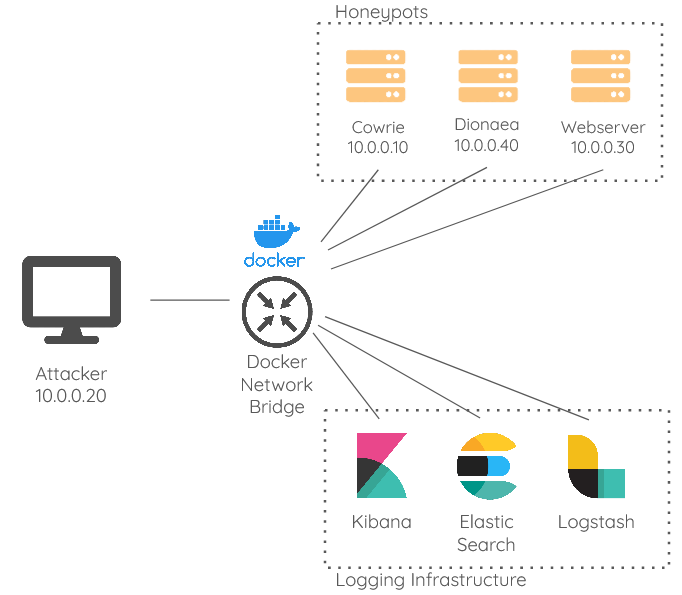
\includegraphics[scale=0.25]{topology}
\end{center}
The docker-compose.yaml file containing the definition for the containers can be found in the netsec-honeypot-lab folder on the desktop or in our Github public repository: 

\url{https://github.com/Marcy-P/netsec-honeypot-lab}

\noindent The repository README also contains additional info for accessing the containers and the references to some Docker images we used.

\section*{Starting up the lab}
To start the laboratory login into the VM with the credentials: username: \textit{netsec} and password: \textit{password}. Then open a terminal in the folder \textbackslash netsec-honeypot-lab on the desktop and type the following command:

\begin{lstlisting}[language=bash]
$ ./start.sh
\end{lstlisting}

\section*{Shutting down the lab}
To shut down the docker-compose network type:

\begin{lstlisting}[language=bash]
$ docker-compose down
\end{lstlisting}

\noindent To also clean the persistent data present in Elasticsearch type:

\begin{lstlisting}[language=bash]
$ docker-compose down -v
\end{lstlisting}

\chapter{What is a honeypot?}
\label{cha:intro}

"A honeypot is a network-attached system set up as a decoy to lure cyber attackers and detect, deflect and study hacking attempts to gain unauthorized access to information systems"\cite{techtarget}. So it is a system that is unprotected and serves no business purpose but sits in the network waiting to be contacted. Every interaction with a honeypot is suspicious because no legitimate user should utilize it.

\chapter{Characteristics of a honeypot}
\label{cha:characteristics}

Honeypots have four main characteristics; they have to be: \textbf{Deceptive} , \textbf{Discoverable}, \textbf{Interactive}, \textbf{Monitored}.

\section{Deception}

Deception can be defined as an advantageous distortion of an adversary's perceptions of reality. Honeypots heavily use this concept as a tool because they appear as real systems, but they do not serve any functional purpose for a business.

There are various frameworks that try to classify various deception strategies, and we considered the taxonomy proposed by Bell and Whaley \cite{Whaley}. According to this model deception consists in two main parts: hiding the real (dissimulation) and showing the false (simulation).

Honeypots are meant to be reachable, so you do not hide it entirely, but you often have to hide specific features of them to make them less suspicious.
The techniques to hide the real are:
\begin{itemize}
\itemsep0em 
\item \textbf{Masking}: hide the  real by making relevant objects be undetectable or blend into the background;
\item \textbf{Repackaging}: hide the  real by making it appear like it is something different;
\item \textbf{Dazzling}: hide the real by altering an object to confuse the adversary;
\end{itemize}

The techniques to show the false are:
\begin{itemize}
\itemsep0em 
\item \textbf{Mimicking}: show the false by using characteristics present in the actual real object;
\item \textbf{Inventing}: show the false by giving the perception that a relevant object exist while it does not; 
\item \textbf{Decoying}: show the false by misdirecting and attracting the attacker attention away from real objects.
\end{itemize}
Note that not every honeypot has to strictly follow these techniques. It is just a theoretical framework that you may want to use when creating and deploying a honeypot. 

\section{Discoverability}
Honeypots are not meant to be accessed by legitimate users but just the attacker. So when designing your honeypot you have to consider the point of view of the attacker.
In particular, you can ask yourself the following questions:
\begin{itemize}
\item Where is the attacker more likely to enter your network?
	\begin{itemize}
	\item User workstations
	\item Vulnerable services exposed to the internet
	\item Stolen VPN credentials
	\end{itemize}
\item What tool will they use to discover your asset?
\item What assets will they be interested in?
\end{itemize}

To increase discoverability, you might also place \textbf{breadcrumbs} in systems that might be compromised. They are data that will lead the attacker to your honeypot while the attacker is gathering information needed to do lateral movement in the network. An example of breadcrumbs is a clear text document containing an URL or IP of a honeypot and some credential or SSH private keys.

\section{Interactivity}

Technically a single attacker interaction is enough to produce an alert. But is better if the honeypot responds back to the attacker for two main reasons:
\begin{itemize}
\item Each interaction that attacker does with the honeypot could provide you important information. For example, if they stole some credential, you may be able to know the account that was compromised. You may be able to find out what tool they use to enter  your network
\item Make the attacker waste time. Every second that the attacker spends interacting with the honeypot is a second you can invest into finding out which systems were compromised and isolate the attacker
\end{itemize}



\section{Monitoring}

Finally, honeypots have to be monitored. This means that every notable interaction with a honeypot must generate an event or alert. This alert generally gets fed to a central SIAM that is accessible to the network administrator or security team.

To manage all the event generated in an environment with multiple honeypots, you have to build a \textbf{logging and monitoring infrastructure} that stores the logs and alerts the analyst of the presence of an attack. The process of shipping logs from the honeypot to the monitoring server usually happens in four phases:
\begin{enumerate}
\item \textbf{Source}: the data are generated from the honeypot. Note that each honeypots produce logs in their own format. You need to be aware of such format because often it is not compatible with the Logging and Monitoring Server.
\item \textbf{Egress}: the data are transmitted to a central location. There has to be a sender capable of reading the logs and sending them to another location. In this phase you also can do some filtering  if some of the information provided in the logs are not needed or conversion to other formats. 
NB: Since you are transferring data over the network you have to consider all the CIA properties because the logs are sensitive data. If you do not encrypt data, you are vulnerable to various attacks that we already see in other laboratories. Can you guess some of them? ARP cache poisoning and MITM. If the attacker can intercept the logs, it can know that a system is a honeypot without never interacting with it!

\item	\textbf{Ingress}: the data are received. There should be a component that receives logs and parses them in a format compatible with the destination. In this phase it is also important to do additional filtering because  some honeypots are very noisy. You may want to filter out interaction that are not important [e.g., not log whey they interact for the first time with the honeypot but just when they authenticate] or interaction from component of the network that may interact with the honeypot (e.g., scanners)
\item \textbf{Destination}: The data are stored in the destination inside a database.  You also can implement a dashboard to see them. This component must be protected because like already said these logs are sensitive data. You may also want a system to backup important logs.
\end{enumerate}

Another mechanism that you can implement in parallel to the logging infrastructure is a monitoring infrastructure. You do not want to miss an attack because a honeypot was down because of a crash. This infrastructure allows to keep track of the status of each honeypot and alert you when a honeypot goes down.

\chapter{Honeypots classification}


\section{Based on level of interaction}

Honeypots are classified by their degree of interaction with the communication destination (attacker) as a low interaction, medium interaction or  high interaction type. However, this does not mean that the high interaction type is better than the low interaction type. These terms are used in different ways depending on implementation, usage and purpose.
\begin{itemize}
\item Low interaction: low interaction honeypots capture the information about the predetermined activities of attackers, and limit these activities by using emulation software. They exclusively utilize emulation software and its services, hence the quality of these honeypots is decided by the quality of emulation software. They are easier to maintain and deploy, and are also more secure compared to high interaction honeypots, because the attacker’s action is limited in the emulated area of the computer. Nonetheless, because it does not imitate the actual OS or application completely, the attacker may notice this machine as a honeypot. 

\item High interaction: high interaction honeypots allow the attackers interacting with real systems and do not assume anything about the possible behavior of the attacker. They help the administrator to investigate the complete activities of the attackers, utilizing the operating systems (eg Linux) and applications (eg FTP) without using the emulation software (eg dionaea) to record the activities of attackers. In most cases attackers are unable to recognize the honeypot because it behaves similarly to the actual target host. However these systems require more resources and are difficult to set up and maintain; also the possibility of infection from the malware or hacking by the attacker is higher than for the low interaction type honeypot. Therefore, the system should be monitored properly, and it is necessary to be prepared to restore the system to the state before the infection of malware.
\item medium-interaction honeypots are a combination of low-interaction and high-interaction honeypots, capable of emulating full services or specific vulnerabilities. Similar to low-interaction honeypots, their primary purpose is detection and are installed as an application on the host operating system with only the emulated services being presented to the public. The key feature of a medium-interaction honeypot is application layer virtualization. They do not aim at simulating a fully operational system environment, nor do they implement all details of an application protocol. They provide sufficient responses that known exploits waiting on certain ports will be tricked into sending their payload. Once this payload has been received, the shellcode can be extracted and analyzed. The medium-interaction honeypot then emulates the actions the shellcode would perform to download the malware.
 
\end{itemize}

\section{Based on the goal}

\begin{itemize}
\item Research honeypots: these are deployed by various security researchers to assess cyber threats, study the real motivation behind the attacks and capture various zero-day exploits. They help in gathering information about attacks and what kind of hacking (attacking) techniques are being used by the attackers. Various logging tools are used to log each and every activity happening on the honeypot, which can really help researchers to study the various advanced methodologies used by an attacker. They mainly consist of high interaction honeypots, in fact they are complex to deploy and maintain.

\item Production honeypots: these are deployed by organizations to mitigate threats and protect themselves from various attacks. They require less resources and can be easily deployed. Production honeypots are often placed near security assets, in order to alert defenders of an attack; they are cheap and usually belong to the low interaction type. Use of low interaction type includes port scan identification, generation of attack signatures, trend analysis and malware collection. On the other hand, this is also a disadvantage, indeed it is not possible to watch how an attacker interacts with the operating system as all the services are emulated.

\end{itemize}

\chapter{Advantages of honeypots}
Honeypots present certain advantages over other defense systems, which is why they should be considered in the development of a well-secured network.

Firstly they consume few resources, especially if compared to traditional IDSs. While an IDS may have to handle gigabytes of data per second, a honeypot has just to handle the activities directed to itself. But it’s important to remember that honeypots are not a substitute for IDS, because usually honeypots are more a reactive control, whereas IDSs act more as preventive controls. Also IDSs deal with known threats (but not only) while honeypots deal with unknown one.

A second advantage is the fact that they are simple and cheap  to maintain. Especially for those belonging to the low interaction type, you can prepare a script that can deploy hundreds of honeypots in your network.

As a third advantage they produce a small number of logs with few false positives, because there is no reason for legitimate users to access the honeypot. So you do not need a whole team of security experts that have to keep checking alerts.

\chapter{Cowrie}

\section{What is Cowrie?}

Cowrie is an open-source medium interaction SSH, and Telnet honeypot designed to log brute force attacks and the shell interaction performed by the attacker \cite{whatcowrie}.
It can run in two modes:
\begin{itemize}
\itemsep0em 
\item In Medium interaction mode (shell) it emulates a UNIX system. To do so it provides:
	\begin{itemize}
	\itemsep0em 
	\item An authentication mechanism via SSH
	\item A  post authentication shell
	\item The ability to create fake file system with files that attacker can cat
	\item A mechanism to save files downloaded inside the shell with wget, curl or uploaded with SFTP and scp
	\end{itemize}
\item In High interaction mode (proxy) it functions as an SSH and telnet proxy to observe attacker behaviour to another system. To use this mode you have to provide a real secure backend environment where the attacker can execute any Unix command.
\end{itemize}

\noindent In this lab we will just focus on the Medium interaction mode because is the most popular one and can be used easily inside a virtual machine.


\section{Start-up Cowrie}
To enter in the Cowrie Docker instance open a terminal in the \textit{netsec-honeypot-lab} folder and type:
\begin{lstlisting}[language=bash]
$  ./startup/cowrie.sh
\end{lstlisting}
Cowrie is already installed and you can start it by typing:
\begin{lstlisting}[language=bash]
$ cowrie start
\end{lstlisting}
You will find the logs in the folder \texttt{var/log/cowrie/cowrie.log}. To print them as they get generated execute the following command:
\begin{lstlisting}[language=bash]
$ tail -f var/log/cowrie/cowrie.log
\end{lstlisting}

\section{Brief exercise - The attacker point of view [4-5 minutes]}
Enter in the attacker machine by typing in another terminal:
\begin{lstlisting}[language=bash]
$ ./startup/attacker.sh
\end{lstlisting}
As the attacker, you successfully installed nmap on the compromised machine and identified a host with the IP 10.0.0.10 (Cowrie IP address). Try to execute a probe scan to see what services run on that host. You can do it with the command:
\begin{lstlisting}[language=bash]
$ nmap -sV 10.0.0.10
\end{lstlisting}
You should see that with the Cowrie default configuration the (fake) SSH service run on port 2222.
Now you should try to connect using common credential for example username: \textit{root} and password: \textit{password}. To do that type the command:
\begin{lstlisting}[language=bash]
$ ssh root@10.0.0.10 -p2222
\end{lstlisting}
Once you are logged in inside the honeypot, play a bit in it and list some strange behaviours you encountered that suggest you that the system is a honeypot.
Things to keep in mind:
\begin{enumerate}
\itemsep0em 
\item With the default configuration there is a time-out that will log you out every two minutes
\item While inside the honeypot don't worry about breaking things.
\item If you get stuck for some reason type in the cowrie terminal: \$ cowrie stop and then start it again.
\end{enumerate}

\section{Brief exercise - Solution}
Here a list of behaviour you may have encountered:
\begin{itemize}
\itemsep0em 
\item If you type the command:
	\begin{lstlisting}[language=bash]
$ uname -v
	\end{lstlisting}
	You get that the system is a Debian Linux distribution. So you may want to try to install some software. For example by typing:
	\begin{lstlisting}[language=bash]
$ apt-get install ftp 
	\end{lstlisting}
	But after the installation screen every time you try to execute the newly installed command you will get the error SEGMENTATION FAULT.
\item When you try to \texttt{cat} some files they seem to exist but you will get the error "\textit{No such file or directory}"
\item You cannot kill processes
\item You are able to downloads  file with wget but when you check their size with the command ls -al you see them as 0 Byte files
\item If you delete all the files in the root folder nothing breaks. And if you re-login into the honeypot all the file will return.
\end{itemize}

\section{A consideration about the previous exercise}
Some may think that is not that hard to figure out that the system is a honeypot, but you have to keep in mind that when the attacker is inside the honeypot we already logged every character he typed.
You can actually replay each session of interaction with the command:
\begin{lstlisting}[language=bash]
$ bin/playlog var/lib/cowrie/tty/[session_log_ID]
\end{lstlisting}
And also check the files that the attacker downloaded by checking the following folder:

\begin{lstlisting}[language=bash]
$ ls var/lib/cowrie/downloads/
\end{lstlisting}

\section{Customizing Cowrie}
The honeypot with the default configuration is almost empty, but the goal is to make the attacker believe that it is a legitimate system. In this way you can increase its interaction with the system and gather intel about what is seeking or what tool it uses. To make Cowrie resemble a legitimate system you have to start by modifying the cowrie config files.

The first thing to do is to copy the default configuration file \texttt{cowrie.cfg.dist} in a file named \texttt{cowrie.cfg}, Cowrie will give priority to this file if it exist:
\begin{lstlisting}[language=bash]
$ cd etc
$ cp cowrie.cfg.dist cowrie.cfg
\end{lstlisting}
Now you can access the file with a text editor (e.g. vim or nano) and edit the following sections:
\begin{itemize}
\item Scroll down a bit and change the \texttt{hostname}. You might want to mimic similar server name existing in the network range of the honeypot. Or you can also stand out with something original.
\item Search for timeout to change the interaction and authentication timeouts to a new value
\item Search for \texttt{listen\_endpoints} in the \texttt{[shell]} section (second match of the search) and modify the port from 2222 to 22
\end{itemize}

\noindent NB: for every modification you want to apply remember to restart Cowrie with the command:

\begin{lstlisting}[language=bash]
$ cowrie restart
\end{lstlisting}

\subsection{Modifying the login credentials}
\label{sub:login}
Another fundamental part to customize are the credentials that the attacker can use to SSH into the honeypot. To achieve this copy the file \texttt{userdb.example} to \texttt{userdb.txt}:
\begin{lstlisting}[language=bash]
$ cd etc
$ cp userdb.example userdb.txt
\end{lstlisting}
Inside this file you will find an explanation of the syntax to use.
Try to use generic credentials that can be easily guessed but without raising suspicion.


\subsection{Modifying the process list}
Cowrie allow you to create a list of fake processes that will be printed with the command \texttt{ps}. To do that modify the JSON file at the following path: \texttt{share/cowrie/cmdoutput.json}. The syntax is self explanatory. When you edit it try to remove processes that are not likely to appear in your system and add processes that are running on a real systems


\subsection{Modifying the file system}
Cowrie provide an emulated file system so when an attacker login it will get its own personal copy of this filesystem that will be deleted when they log off. This file system is implemented into two components:
\begin{itemize}
\itemsep0em 
\item \textbf{pickle file}: contains metadata for the files (their name, size, permission, directory, …)
\item \textbf{honeyfs directory}: contains the file contents
\end{itemize}

\noindent NB: to be visible (\texttt{ls}) a file must be in the pickle file, and to be also accessible (\texttt{cat}) it needs to be in the honeyfs directory.

You can find the \texttt{honeyfs} directory in the cowrie installation folder. An interesting file you can modify is \texttt{motd} that contain the SSH post login banner.
\begin{lstlisting}[language=bash]
$ cd honeyfs
$ vim etc/motd
\end{lstlisting}

If you created a new user credentials in the section \ref{sub:login} remember to create also the home directory for that user.
Also, for the next section create a file \texttt{/bin/nmap}.

Finally you can generate the pickle file automatically by typing:
\begin{lstlisting}[language=bash]
$ rm ./share/cowrie/fs.pickle
$ ./bin/createfs -l honeyfs -d 5 -o ./share/cowrie/fs.pickle
\end{lstlisting}
The flag \texttt{-l} is used to specify the location of the honeyfs folder, the flag \texttt{-d} sets the depth of the file system you want to include. Finally the flag \texttt{-o} sets the location of the pickle file you are creating. Cowrie will search for the pickle file in the \texttt{./share/cowrie/} directory.



\subsection{Adding new commands}

To add a new command add a file in the folder \texttt{share/cowrie/txtcmds/bin} containing a static output for that command. Previously we created the binary file for nmap so now you can try to create an output for nmap.
\begin{lstlisting}[language=bash]
$ vim share/cowrie/txtcmds/bin/nmap
\end{lstlisting}
Now when executing the command \texttt{nmap} the attacker will receive the static output you specified.

\chapter{Dionaea}

\chapter{Honeyfiles}

A honeyfile is an intrusion detection mechanism based on deception. This mechanism works by creating a bait file that when accessed set off an alarm or log the access to the document. In this way you can detect unauthorized access to a computer. This is a very simple technique, but it is also very effective. Usually, in many organizations important information gets stored in office documents. So, when an attacker compromises a machine, he often checks for valuable documents.

When “setting up” a honeyfile you have to think about what the attacker is interested in. Usually they search for four things:
\begin{enumerate}
\itemsep0em 
\item Information for accessing other systems (e.g., passwords, network details) or security documentation
\item File containing important information's like intellectual property, customer lists, product design.
\item File containing personal information that could be  used to harm reputation or allow further compromise of the system
\item Log files that can contain evidence of attacks.
\end{enumerate}

Then you have to think what the attacker will see, so:
\begin{itemize}
\itemsep0em
\item You must place the file in a way that can be easily found. But if it is a system used by legitimate users that are unaware of the honeypot, you should place it in a way that is unlikely to be accidentally opened.
\item Is very effective when the file stands out from other files. You can achieve this in various ways:
	\begin{itemize}
	\itemsep0em
	\item FILE NAME IN CAPS
	\item Usage of a document type different from the other documents around it
	\item Setting a unique or odd file size (e.g., a 23 MB word document between 15 kB documents)
	\end{itemize}
\end{itemize}

\noindent NB: Do not exaggerate by placing to many honeyfiles, because it will also increase the chance of triggering false positives by legitimate users. And also do not try to hard with the naming conventions otherwise the attacker will become suspicious.

\section{How to create a honeydoc}


\chapter{Lab monitoring infrastructure}

To implement our logging infrastructure we used the Elastic Stack (also known as ELK stack) an open-source log management system composed of four components:
\begin{enumerate}
\item \textbf{Beat}: is the component that assumes the role of the egress. More technically is a family of lightweight data shippers that can be installed in each honeypot system to send various types of information. For each information there is a specific beat agent, for example:
	\begin{itemize}
	\item \textbf{Filebeat}: it is used to send logs and files. It allows also to parse common logs format. We used this agent to send our honeypot logs to Logstash.
	\item Metricbeat: agent used to ship metric data.
	\item Winlogbeat: to ship windows event logs.
	\item Heartbeat: to ship data regarding uptime monitoring
	\end{itemize}
\item \textbf{Logstash}: assumes the role of the ingress. It receives data from the various Filebeats, parse and filter them. Then sends its output (that is in JSON format) to Elasticsearch. NB: It is very powerful because you can use it to structure unstructured data and enrich them with new information (for example geo coordinates based on the IP address inside a log).
\item \textbf{Elasticsearch}: it is the destination of the data. It receives the data from Logstash, store them  in a database and indexes them. This process allows to run queries on the data and aggregate them into useful information. 
\item \textbf{Kibana}: is a web-based dashboard that is used to visualize the data present in Elasticsearch. It allows you to create real-time histograms, pie charts and maps
\end{enumerate}

\chapter{Honeypots for IoT}
\endgroup


% bibliografia in formato bibtex
%
% aggiunta del capitolo nell'indice
\addcontentsline{toc}{chapter}{Bibliography}
% stile con ordinamento alfabetico in funzione degli autori
\bibliographystyle{plain}
\bibliography{biblio}
\end{document}
